\section{Introduction}
\label{sec:introduction}

% state the learning objective 
The objective of this laboratory assignment is to analyse and optimize an audio amplifier circuit, with a $12V$ supply voltage (Vcc) and an audio input of up to $10mV$, using a gain and an output stage, as presented in Figure  \ref{fig:circ}. In order to optimize the circuit, it was possible to manipulate the values of several parameters, which had assigned costs, given by the Professor.. The \textit{Merit} score is obtained as a function of the chosen architecture's cost and the performance of the circuit. 


\begin{figure}[h] \centering
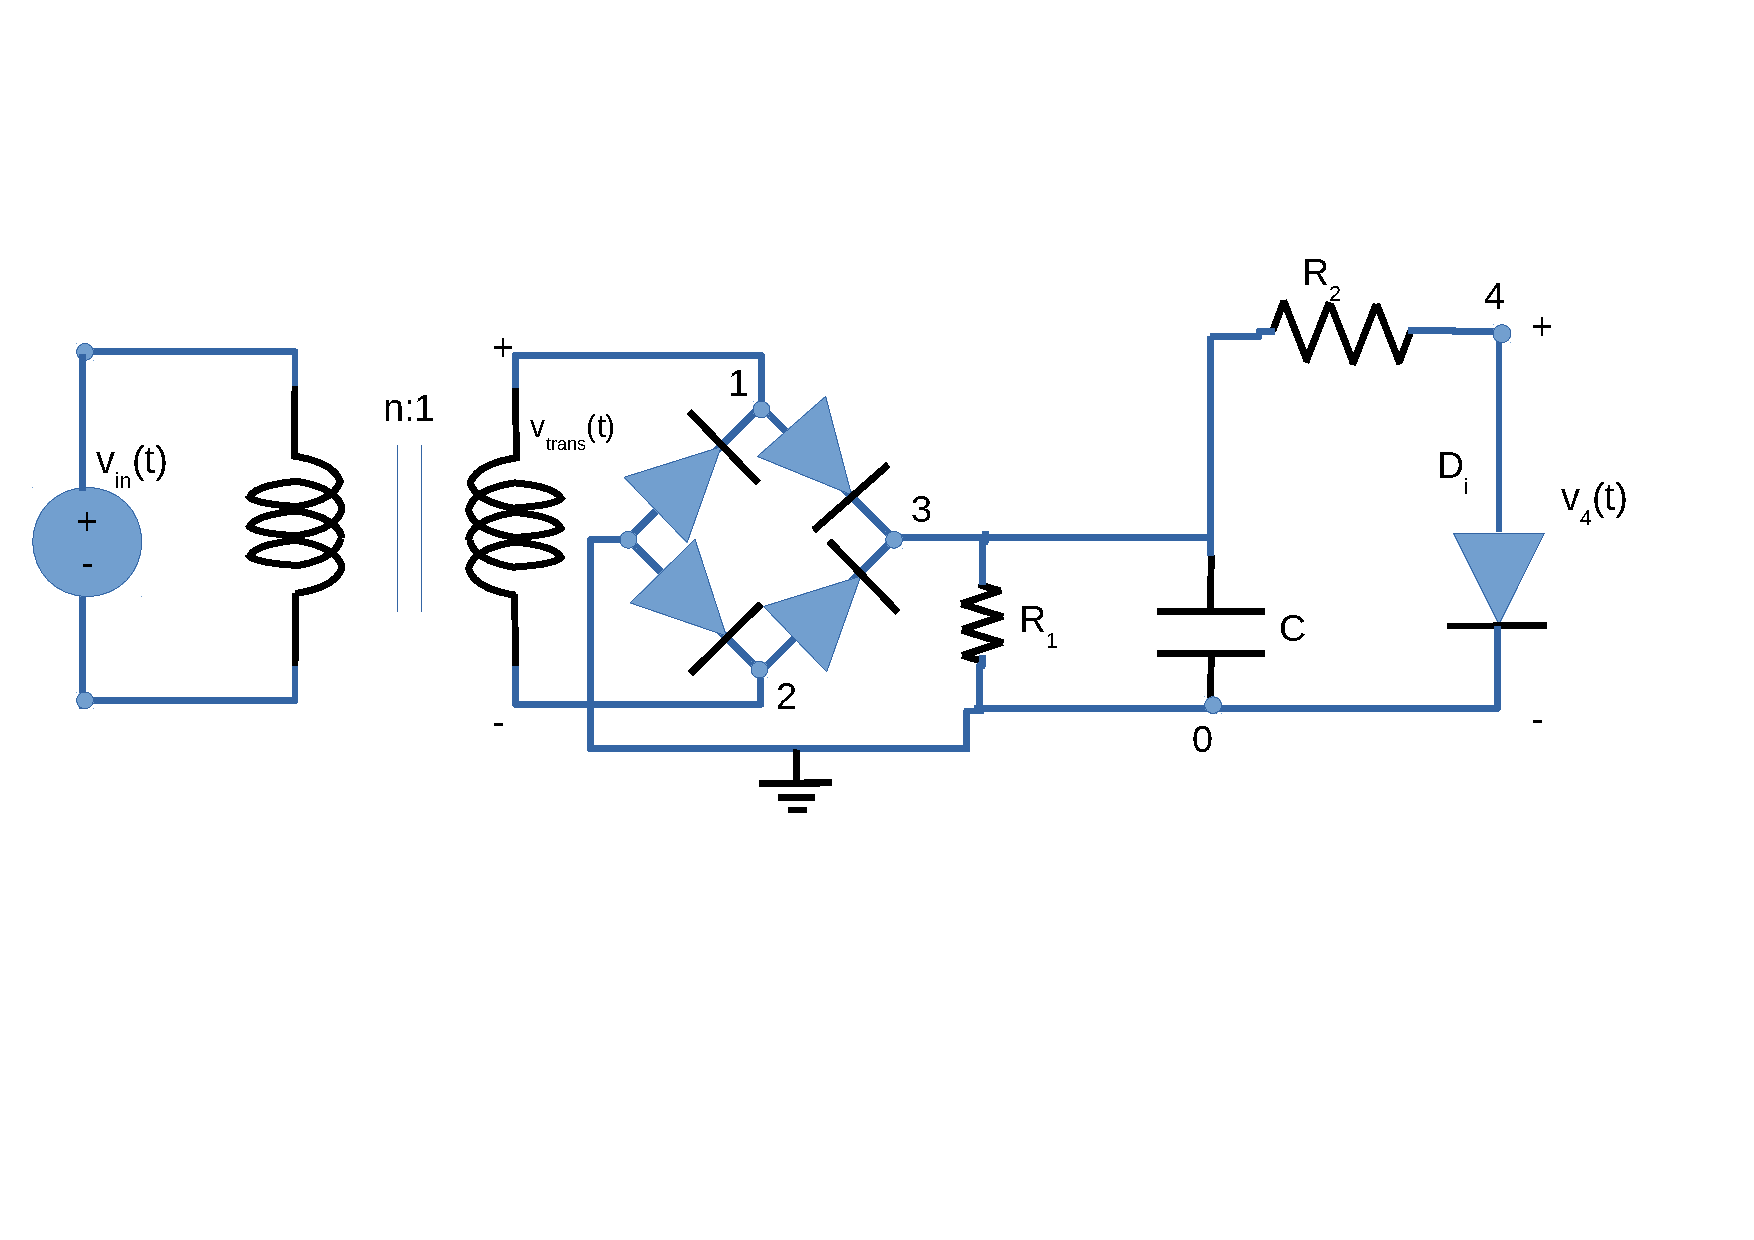
\includegraphics[width=0.9\linewidth]{circ.pdf}
\caption{Audio amplifier circuit.}
\label{fig:circ}
\end{figure}

in which $R_1 = 20000 \si{\ohm}$, $C=0.00001 F$, $R_2 = 2000 \si{\ohm}$, $n=17$, <- mudar isto para os valores e arquitectura usada.
The cost of the architecture is !!!!!!


In Section~\ref{sec:analysis}, using \textit{Octave}, a theoretical analysis is presented, in which we describe the theoretical model used to analyze the circuit are presented. In this Section's last subsection (Subsection \ref{subsec:theo_merit}), the cost of the circuit and Merit score are determined. In Section~\ref{sec:simulation}, the circuit is analyzed by simulation, but using the Ngspice software. The results are compared in Subsection~\ref{subsec:compare} (the last of this third Section). The conclusions of this study are outlined in Section~\ref{sec:conclusion}.